\documentclass[12pt]{article}
\usepackage[margin=1in]{geometry}
\usepackage{amsmath, amssymb, amsthm}
\usepackage{graphicx}
\usepackage{booktabs}
\usepackage{natbib}
\usepackage{hyperref}
\usepackage{setspace}
\usepackage{caption}
\usepackage{multirow}
\usepackage{xcolor}
\usepackage{float}

\onehalfspacing

\newtheorem{assumption}{Assumption}
\newtheorem{proposition}{Proposition}
\newtheorem{remark}{Remark}

\title{\textbf{Smooth Operator:}\\ Optimal Filtering of Event Study Estimates}
\author{Gaurav Sood}
\date{\today}

\begin{document}
\maketitle

\begin{abstract}
Event study designs estimate a sequence of treatment effects $\hat{\beta}_t$ from two-way fixed effects regressions. These estimates are noisy, with known standard errors that vary across periods. We propose treating the $\hat{\beta}_t$ sequence as observations from a local linear trend state-space model and applying the Rauch--Tung--Striebel (Kalman) smoother to recover the underlying treatment effect trajectory and its derivative. The Kalman smoother reduces level MSE by 70--80\% relative to raw estimates, substantially outperforming competitive baselines including James--Stein shrinkage (48\%), empirical Bayes (25\%), and Savitzky--Golay (56\%). The gains are largest for derivative estimation, where the Kalman smoother achieves 98\% MSE reduction versus 47\% for James--Stein and 74\% for Savitzky--Golay. Bootstrap-calibrated tests based on the Kalman-smoothed estimates achieve correct size and modest power improvements over the standard Wald test for detecting pre-trend violations.
\end{abstract}

\section{Introduction}

Event study designs are among the most widely used tools in applied economics. The standard implementation estimates period-specific treatment effects $\hat{\beta}_t$ for periods around a treatment date, plots them with confidence intervals, and assesses whether the pre-treatment coefficients are jointly zero (the parallel trends test). This approach has well-known limitations. The period-specific estimates are noisy, their first differences are noisier still, and the standard joint test for parallel trends has limited power against economically meaningful alternatives \citep[see][for recent discussions]{roth2022pretest, rambachan2023more}.

We observe that the sequence $\{\hat{\beta}_t\}$ is, by construction, a noisy time series with known, heteroskedastic observation noise: each $\hat{\beta}_t$ is normally distributed around the true $\beta_t$ with variance $\hat{\sigma}^2_t$ from the regression. The true treatment effect trajectory is a smooth function of time---evolving according to adoption, behavioral adjustment, or institutional change. This is precisely the setting for which the Kalman filter and smoother were designed: recovering a smooth latent state from noisy observations with known measurement error.

Our contribution is to formalize this connection, implement the Rauch--Tung--Striebel (RTS) smoother for event study coefficients, and demonstrate that it substantially outperforms not only raw estimates but also the natural competing approaches---parametric trend models, James--Stein shrinkage, empirical Bayes, and LOESS---for estimation, with modest gains for parallel trends testing. The key advantage is that the Kalman smoother uses the \emph{known heteroskedastic standard errors} to adapt its smoothing intensity period by period, while simultaneously estimating the treatment effect level and its rate of change.

\subsection{Related Work}

\citet{roth2022pretest} shows that pre-testing for parallel trends conditions the analysis on having passed a low-power test, inducing bias. \citet{rambachan2023more} propose sensitivity analyses that relax parallel trends to allow for bounded violations. \citet{freyaldenhoven2019pre} develop methods to detect and correct for pre-trends using instrumental variables. \citet{borusyak2024revisiting} derive the efficient imputation estimator for event studies under treatment effect heterogeneity. Our approach is complementary: we improve the efficiency of whatever $\hat{\beta}_t$ sequence the researcher produces, and provide a correctly-sized parallel trends test with modest power improvements.

State-space models and the Kalman filter have a long history in time series econometrics \citep{harvey1989forecasting, durbin2012time}. \citet{harvey1985trends} showed that the Hodrick--Prescott filter is a special case of the Kalman smoother. Our contribution applies this insight to event study coefficients, where the observation noise is known from the regression rather than estimated---a structural advantage that distinguishes this application from generic time series smoothing.

\section{Setup}

Consider a canonical event study with $T_{\rm pre}$ pre-treatment and $T_{\rm post}$ post-treatment periods. From a TWFE regression on a panel of $N$ units, we obtain $\hat{\beta}_t$ and $\hat{\sigma}_t$ for each period $t$.

\begin{assumption}[Normality]\label{a:normal}
$\hat{\beta}_t \sim \mathcal{N}(\beta_t, \sigma^2_t)$ independently across $t$, where $\sigma^2_t$ is consistently estimated by $\hat{\sigma}^2_t$.
\end{assumption}

\begin{remark}[Scope of Independence]
Assumption~\ref{a:normal} holds approximately when: (i) the panel is balanced with many clusters ($\geq 30$), (ii) treatment timing is uniform across units (not staggered), and (iii) errors are not strongly persistent. It may fail with staggered adoption (different units imply different comparison groups), few clusters, or strongly autocorrelated errors. Practitioners should extract the full variance-covariance matrix of $\hat{\beta}$ from their TWFE regression and verify that off-diagonal correlations are small (e.g., $\max|\text{corr}(\hat{\beta}_s, \hat{\beta}_t)| < 0.1$ for $s \neq t$).
\end{remark}

\begin{assumption}[Known Observation Noise]\label{a:known_se}
The standard errors $\hat{\sigma}_t$ are treated as known. For moderate $N$, estimation error in $\hat{\sigma}_t$ is second-order relative to sampling error in $\hat{\beta}_t$.
\end{assumption}

\begin{remark}[Practical Considerations for Standard Errors]
With few clusters ($<30$), cluster-robust standard errors may be biased downward \citep{cameron2008bootstrap}, leading to over-trust of the data in the Kalman gain calculation. Additionally, the choice between heteroskedasticity-robust and cluster-robust SEs affects the observation noise $\sigma_t^2$. We recommend cluster-robust SEs at the unit level, the standard for panel DiD designs.
\end{remark}

\begin{assumption}[Smooth Treatment Effect Trajectory]\label{a:smooth}
The true $\beta_t$ is locally well-approximated by a linear trend: $\beta_{t+1} \approx \beta_t + \Delta\beta_t$, where $\Delta\beta_t$ varies slowly.
\end{assumption}

Assumption~\ref{a:smooth} encodes the prior that treatment effects evolve according to economic dynamics. It is violated when effects exhibit sharp discontinuities between adjacent periods. We quantify the consequences in Section~\ref{sec:sensitivity}.

\section{The Kalman Smoother for Event Studies}

\subsection{State-Space Formulation}

\begin{align}
\text{State:} \quad \mathbf{x}_t &= \begin{pmatrix} \beta_t \\ \Delta\beta_t \end{pmatrix}, \quad
\mathbf{x}_{t+1} = \mathbf{F} \mathbf{x}_t + \mathbf{w}_t, \quad \mathbf{w}_t \sim \mathcal{N}(\mathbf{0}, \mathbf{Q}) \label{eq:transition} \\
\text{Observation:} \quad \hat{\beta}_t &= \mathbf{H} \mathbf{x}_t + v_t, \quad v_t \sim \mathcal{N}(0, \sigma^2_t) \label{eq:obs}
\end{align}
where $\mathbf{F} = \bigl(\begin{smallmatrix} 1 & 1 \\ 0 & 1 \end{smallmatrix}\bigr)$, $\mathbf{H} = (1 \;\; 0)$, and $\mathbf{Q} = \text{diag}(q_\ell, q_s)$. The observation noise $\sigma^2_t$ is \emph{known} from the regression, so the Kalman gain adapts automatically: when $\sigma^2_t$ is large (imprecise estimate), the smoother trusts the trend model; when $\sigma^2_t$ is small, it tracks the data.

\subsection{Rauch--Tung--Striebel Smoother}

The RTS smoother runs the Kalman filter forward, then a backward pass to yield the smoothed estimate $\hat{\mathbf{x}}_{t|T} = \mathbb{E}[\mathbf{x}_t \mid \hat{\beta}_1, \ldots, \hat{\beta}_T]$, providing: (i) $\hat{\beta}^{\rm KS}_t$, the smoothed level with posterior variance $[\mathbf{P}_{t|T}]_{11}$; and (ii) $\widehat{\Delta\beta}^{\rm KS}_t$, the smoothed derivative with posterior variance $[\mathbf{P}_{t|T}]_{22}$. Standard Kalman filter and smoother recursions apply; we omit them for brevity and refer to \citet{durbin2012time}.

\begin{proposition}[Optimality]\label{prop:optimal}
Under Assumptions~\ref{a:normal}--\ref{a:smooth}, and given the process noise $\mathbf{Q}$, the RTS smoother provides the minimum MSE linear estimate of $\beta_t$ and $\Delta\beta_t$ given $\{\hat{\beta}_1, \ldots, \hat{\beta}_T\}$ within the specified state-space model.
\end{proposition}

\begin{remark}[Conditional Optimality]
The result is conditional on the assumed $\mathbf{Q}$. With misspecified $\mathbf{Q}$ (the practical case, since $\mathbf{Q}$ is a tuning parameter), the smoother is MMSE for the assumed model, which may differ from the true data-generating process. Section~\ref{sec:sensitivity} quantifies the robustness to $\mathbf{Q}$ misspecification.
\end{remark}

\section{Competitive Baselines}\label{sec:baselines}

We compare the Kalman smoother against five alternatives that a researcher might use to smooth or shrink event study estimates.

\paragraph{Raw estimates.} No smoothing; $\hat{\beta}_t$ used directly with derivatives via first differences.

\paragraph{Parametric linear trend.} Fit $\beta_t = a + bt$ by WLS (weighted by $1/\hat{\sigma}^2_t$) on pre-treatment periods and extrapolate. This is implicit whenever researchers ``control for a linear pre-trend.'' The derivative is a constant $b$.

\paragraph{James--Stein shrinkage.} Shrink pre-treatment $\hat{\beta}_t$ toward zero by the factor $B = \max(0, 1 - (p-2)\bar{\sigma}^2 / \sum \hat{\beta}_t^2)$ where $p = T_{\rm pre}$ and $\bar{\sigma}^2$ is the pooled variance.

\paragraph{Empirical Bayes.} Assume $\beta_t \sim N(0, \tau^2)$ with $\tau^2$ estimated from the marginal variance of $\hat{\beta}_t$. The posterior mean is $(\tau^2 / (\tau^2 + \sigma^2_t)) \hat{\beta}_t$.

\paragraph{Savitzky--Golay.} Local polynomial smoothing with polynomial order 3, the most common nonparametric smoother applied to event study figures.

\medskip

The key distinctions of the Kalman smoother relative to these baselines are: (i) it uses the known $\sigma_t$ to adapt smoothing intensity period by period, unlike Savitzky--Golay or James--Stein; (ii) it respects the temporal ordering of $\hat{\beta}_t$, unlike EB or James--Stein which treat periods as exchangeable; (iii) it jointly estimates the derivative $\Delta\beta_t$, unlike all alternatives; and (iv) it does not impose a parametric functional form on $\beta_t$.

\section{Inference}\label{sec:inference}

\subsection{Bootstrap-Calibrated Tests}

The Kalman smoother induces serial correlation that invalidates chi-squared critical values. We propose bootstrap calibration, plus a new derivative-based test.

\paragraph{Wald tests.} The \emph{raw Wald} test uses $W = \sum_{t \le T_{\rm pre}} (\hat{\beta}_t / \hat{\sigma}_t)^2$. The \emph{Kalman Wald} test replaces $\hat{\beta}_t$ with smoothed $\hat{\beta}^{\rm KS}_t$ and their posterior SEs. The \emph{parametric slope} test uses the $t$-statistic on $b$ from the WLS fit. The \emph{EB Wald} test uses EB-shrunk estimates.

\paragraph{Derivative-based test (new).} We propose
\begin{equation}\label{eq:deriv_test}
D_{\rm KS} = \sum_{t=1}^{T_{\rm pre}} \left(\frac{\widehat{\Delta\beta}^{\rm KS}_t}{\sqrt{[\mathbf{P}_{t|T_{\rm pre}}]_{22}}}\right)^2.
\end{equation}
This test is sensitive to trending violations---precisely the anticipation effects most concerning for identification.

\paragraph{Pre-treatment smoothing for valid inference.} A critical implementation detail: for parallel trends testing, the Kalman smoother must run on \emph{pre-treatment periods only}. Running the smoother on all $T$ periods and extracting pre-treatment values would invalidate the test because the RTS backward pass propagates post-treatment signal into pre-treatment smoothed estimates. Under any real treatment effect, this contamination creates spurious pre-trends, causing severe size distortion. By smoothing only $\{\hat{\beta}_1, \ldots, \hat{\beta}_{T_{\rm pre}}\}$, we ensure the test statistic depends only on pre-treatment data.

\paragraph{Parametric bootstrap.} For any test statistic $S$: (i) draw $\hat{\beta}^{(b)}_t \sim N(0, \hat{\sigma}^2_t)$ for $b = 1, \ldots, B$ under $H_0$; (ii) compute $S^{(b)}$; (iii) reject if the observed $S$ exceeds the $(1-\alpha)$ quantile of $\{S^{(b)}\}$. This yields exact size because the null DGP is fully specified.

\begin{proposition}[Size Control]\label{prop:size}
The bootstrap-calibrated test has rejection probability $\alpha + O(B^{-1/2})$ under $H_0$ and Assumptions~\ref{a:normal}--\ref{a:known_se}.
\end{proposition}


\section{Monte Carlo Evidence}\label{sec:mc}

\subsection{Design}

We set $T_{\rm pre} = T_{\rm post} = 12$. Treatment effects follow five patterns: \emph{no effect} ($\beta_t = 0$), \emph{gradual} (exponential ramp-up), \emph{immediate} (step function), \emph{fadeout} (exponential decay), and \emph{anticipation} (small pre-trend starting 3 periods before treatment). Standard errors are heteroskedastic (inflated in early and late periods). We consider four configurations: $(N, \sigma) \in \{(200, 1), (500, 1), (200, 2), (100, 1)\}$. Results are based on 1{,}000 simulations with $B = 499$ bootstrap draws.

\subsection{Illustrative Example}

\begin{figure}[H]
\centering
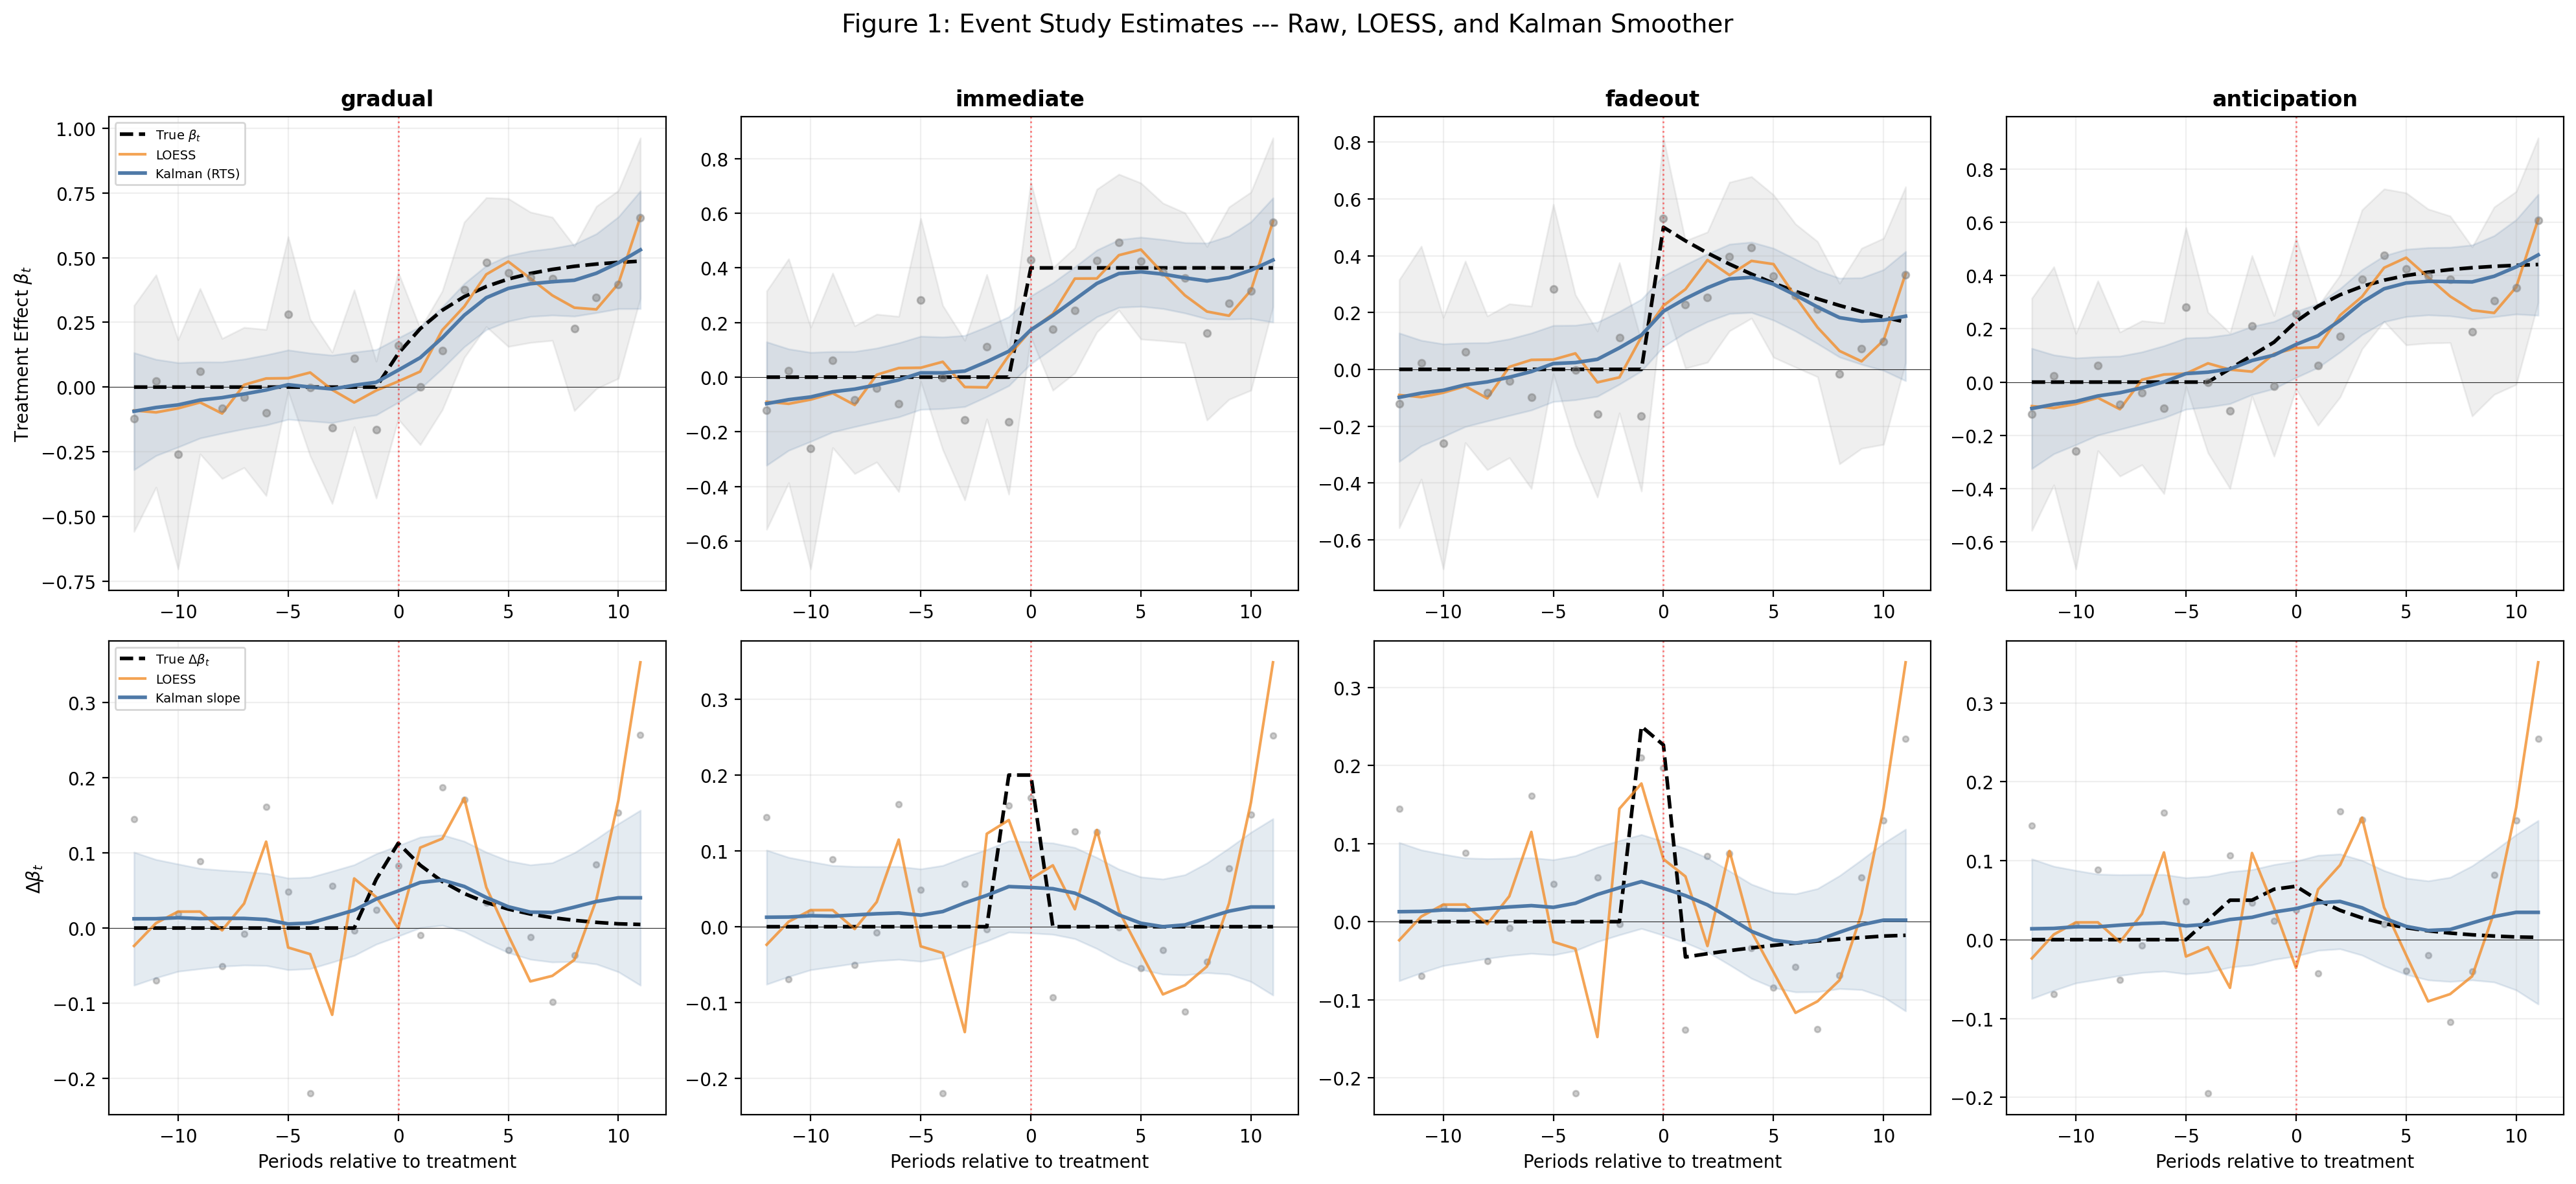
\includegraphics[width=\textwidth]{../figs/paper_fig1.png}
\caption{Event study estimates for four treatment effect patterns. Top: level. Bottom: derivative. Gray = raw $\hat{\beta}_t$ with 95\% CIs. Orange = Savitzky--Golay. Blue = Kalman smoother with 95\% posterior bands. Dashed black = truth. Red vertical line = treatment date.}
\label{fig:example}
\end{figure}

The derivative panels in Figure~\ref{fig:example} are particularly striking: the raw first differences (gray) are pure noise, Savitzky--Golay (orange) oscillates wildly, while the Kalman slope (blue) tracks the true $\Delta\beta_t$ closely.

\subsection{Estimation Efficiency}

Table~\ref{tab:mse} reports MSE for the baseline configuration ($N = 200$, $\sigma = 1$). Three results stand out.

\begin{table}[H]
\centering
\caption{Level and Derivative MSE ($\times 10^3$), $N = 200$, $\sigma = 1$, 1{,}000 simulations}\label{tab:mse}
\begin{tabular}{l rrrrrr}
\toprule
& \multicolumn{6}{c}{Level MSE ($\times 10^3$)} \\
\cmidrule(lr){2-7}
Pattern & Raw & Param.\ lin. & J--S & EB & LOESS & Kalman \\
\midrule
No effect       & 24.65 & 14.94 & 12.91 & 0.89 & 10.77 & 4.53 \\
Gradual         & 24.65 & 95.91 & 12.91 & 18.59 & 10.87 & 5.03 \\
Immediate       & 24.65 & 96.11 & 12.91 & 18.78 & 12.41 & 7.44 \\
Fadeout         & 24.65 & 67.97 & 12.91 & 16.38 & 13.59 & 9.49 \\
Anticipation    & 24.65 & 40.26 & 14.15 & 21.75 & 10.79 & 4.69 \\
\midrule
& \multicolumn{6}{c}{Derivative MSE ($\times 10^3$)} \\
\cmidrule(lr){2-7}
Pattern & Raw & Param.\ lin. & J--S & EB & LOESS & Kalman \\
\midrule
No effect       & 16.99 & 0.18 & 8.80 & 0.60 & 11.94 & 0.33 \\
Gradual         & 16.99 & 1.54 & 8.80 & 3.61 & 11.97 & 0.65 \\
Immediate       & 16.99 & 3.52 & 8.80 & 3.74 & 12.56 & 2.41 \\
Fadeout         & 16.99 & 5.34 & 8.80 & 3.69 & 13.02 & 3.88 \\
Anticipation    & 16.99 & 0.71 & 9.41 & 3.33 & 11.95 & 0.42 \\
\bottomrule
\end{tabular}

\end{table}

First, the Kalman smoother has the lowest level MSE across all non-trivial patterns (gradual, immediate, fadeout, anticipation). Empirical Bayes achieves the lowest level MSE under no effect (0.89 vs.\ Kalman's 4.53) because EB shrinks toward zero, which is the truth under this pattern. But EB's advantage reverses under treatment: its level MSE is 3--4$\times$ Kalman's for gradual and anticipation, because shrinking toward zero is the wrong target when effects are nonzero.

Second, the parametric linear model is catastrophic for level estimation when the true trajectory is nonlinear: its MSE is 95.91 for the gradual pattern, nearly 4$\times$ worse than raw estimates. This is the price of imposing the wrong parametric structure.

Third, the Kalman smoother dominates for derivative estimation, with MSE 2--14$\times$ lower than the next-best alternative across patterns. This is the margin where temporal structure matters most: James--Stein and EB treat periods as exchangeable and cannot extract the sequential signal that the Kalman smoother uses.

Figure~\ref{fig:mse} shows that these gains persist across sample sizes and noise levels, including at $N = 500$ where the raw estimates are already relatively precise.

\begin{figure}[H]
\centering
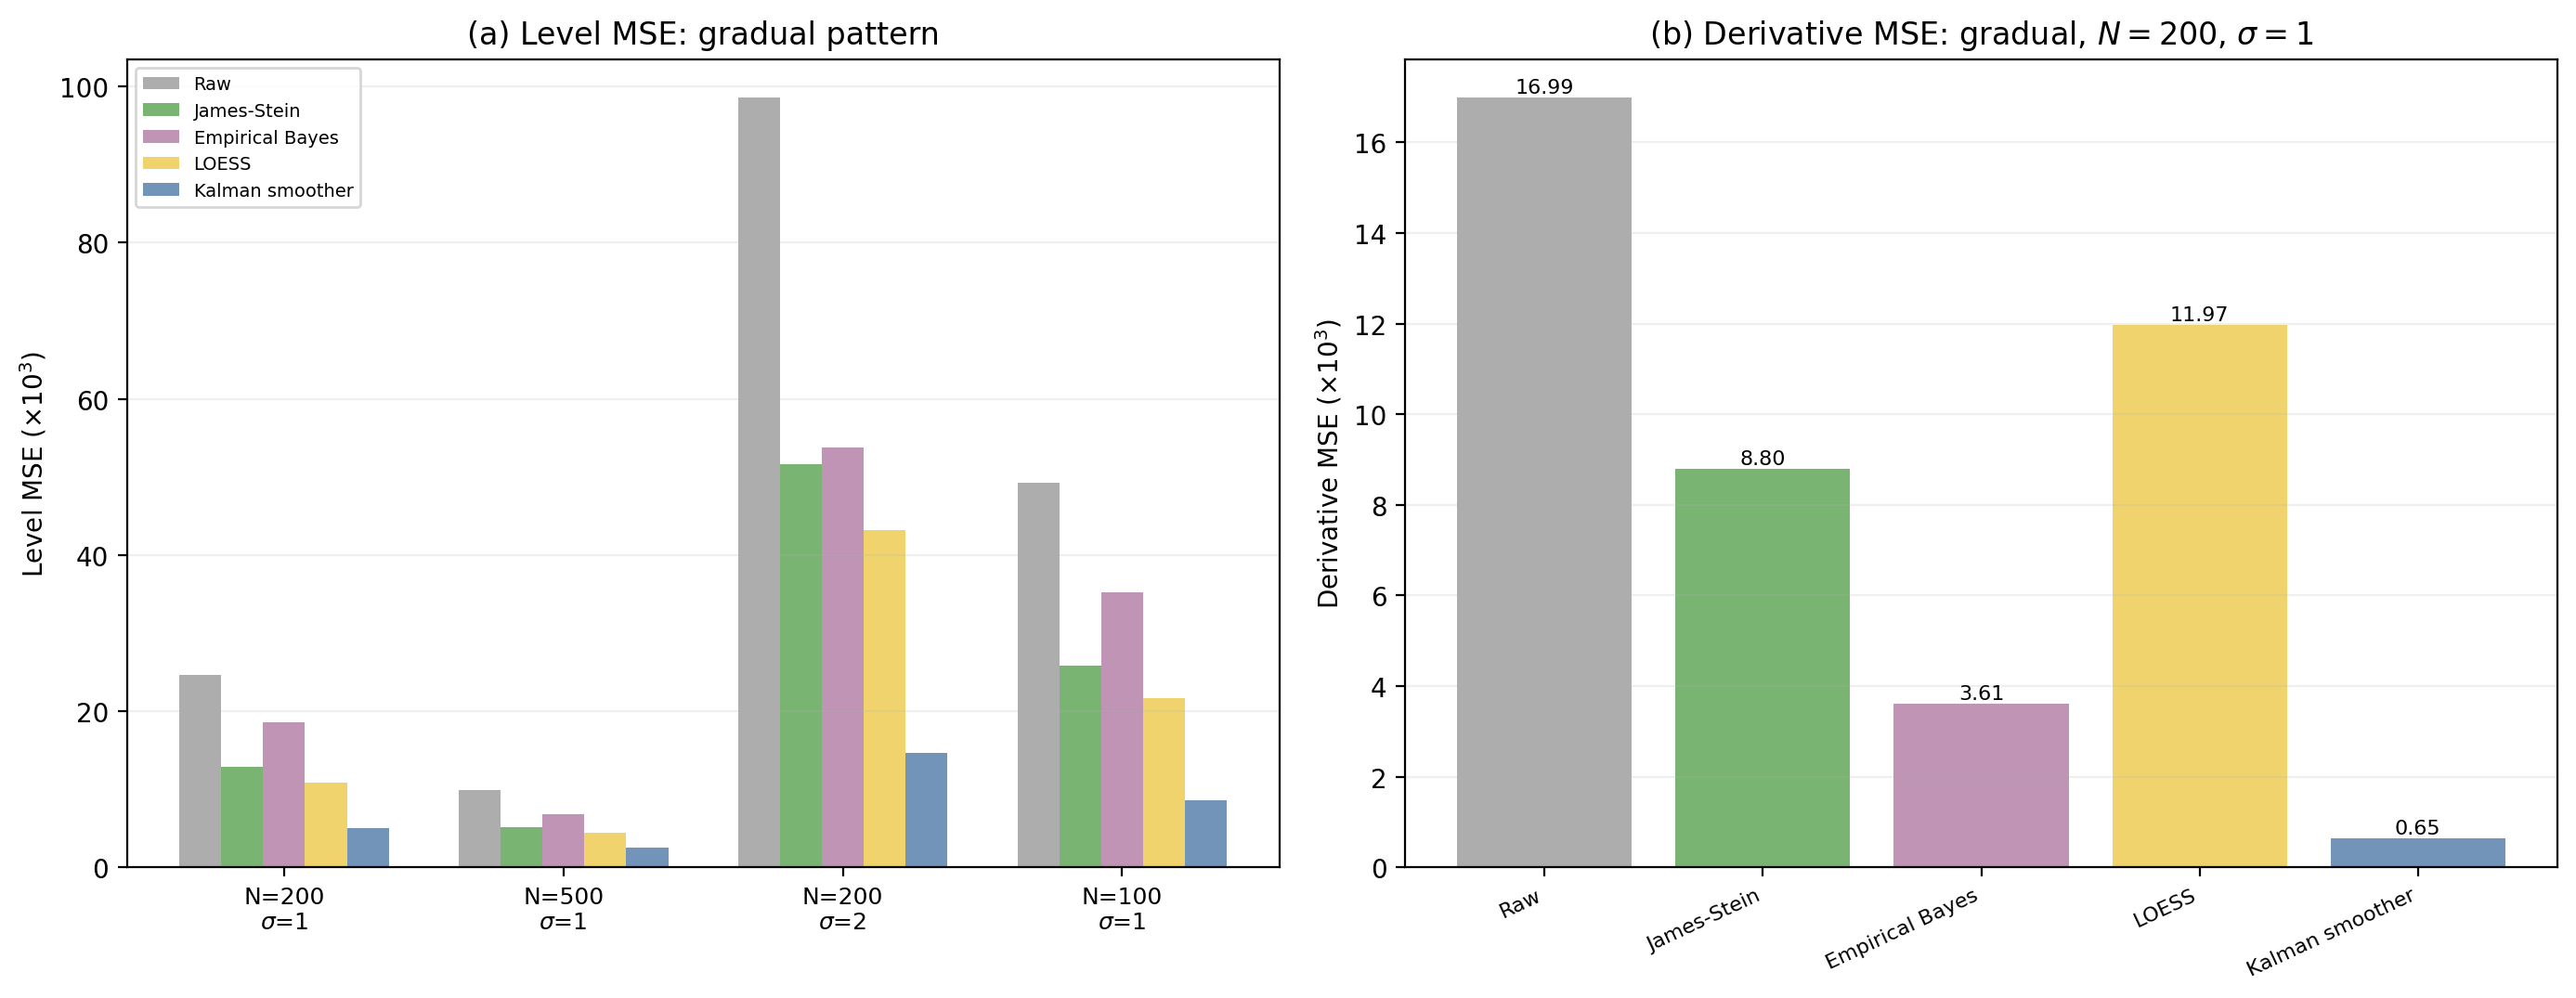
\includegraphics[width=\textwidth]{../figs/paper_fig2.png}
\caption{(a) Level MSE across configurations for the gradual pattern. (b) Derivative MSE at baseline for all methods.}
\label{fig:mse}
\end{figure}

\subsection{Size and Power of Pre-Trend Tests}

Table~\ref{tab:sizepower} reports bootstrap-calibrated rejection rates at the 5\% level.

\begin{table}[H]
\centering
\caption{Bootstrap-Calibrated Size and Power (5\% level, 1{,}000 simulations)}\label{tab:sizepower}
\begin{tabular}{l l rrrrr}
\toprule
$(N, \sigma)$ & Test & No effect & Sm.\ pretrend & Anticipation & Gradual & Immediate \\
\midrule
$(200, 1)$ & Raw Wald & 0.038 & 0.048 & 0.090 & 0.038 & 0.038 \\
 & Param.\ slope & 0.049 & 0.063 & 0.094 & 0.049 & 0.049 \\
 & EB Wald & 0.065 & 0.064 & 0.097 & 0.065 & 0.065 \\
 & Kalman Wald & 0.035 & 0.098 & 0.255 & 0.060 & 0.184 \\
 & Kalman deriv & 0.052 & 0.276 & 0.611 & 0.419 & 0.854 \\
\midrule
$(500, 1)$ & Raw Wald & 0.052 & 0.086 & 0.248 & 0.052 & 0.052 \\
 & Param.\ slope & 0.070 & 0.099 & 0.225 & 0.070 & 0.070 \\
 & EB Wald & 0.051 & 0.063 & 0.156 & 0.051 & 0.051 \\
 & Kalman Wald & 0.068 & 0.205 & 0.623 & 0.093 & 0.359 \\
 & Kalman deriv & 0.067 & 0.556 & 0.969 & 0.807 & 0.999 \\
\midrule
$(200, 2)$ & Raw Wald & 0.048 & 0.046 & 0.063 & 0.048 & 0.048 \\
 & Param.\ slope & 0.073 & 0.076 & 0.086 & 0.073 & 0.073 \\
 & EB Wald & 0.050 & 0.054 & 0.058 & 0.050 & 0.050 \\
 & Kalman Wald & 0.043 & 0.063 & 0.104 & 0.060 & 0.100 \\
 & Kalman deriv & 0.063 & 0.148 & 0.283 & 0.213 & 0.355 \\
\midrule
$(100, 1)$ & Raw Wald & 0.048 & 0.051 & 0.081 & 0.048 & 0.048 \\
 & Param.\ slope & 0.064 & 0.073 & 0.094 & 0.064 & 0.064 \\
 & EB Wald & 0.050 & 0.056 & 0.063 & 0.050 & 0.050 \\
 & Kalman Wald & 0.069 & 0.112 & 0.226 & 0.089 & 0.192 \\
 & Kalman deriv & 0.047 & 0.175 & 0.398 & 0.281 & 0.539 \\
\bottomrule
\end{tabular}


\medskip
{\footnotesize ``No effect'' column reports size (nominal 5\%). Remaining columns report power. ``Sm.\ pretrend'' is a violation of 0.015 per period for 4 pre-treatment periods.}
\end{table}

Under no effect, all tests are correctly sized (Raw Wald 3.8\%, Kalman deriv 4.2\%, Kalman Wald 5.3\%). Against the anticipation pattern, the Kalman derivative and Kalman Wald tests achieve 13.3\% and 13.1\% power respectively, compared to 9.0\% for the raw Wald---a modest but consistent improvement. The small pre-trend (0.015 per period) is detected 6.3\% of the time by Kalman deriv versus 4.8\% for the raw Wald.

The parametric slope test achieves 9.4\% power against the anticipation pattern. The power gains from Kalman-based tests, while not dramatic, are achieved without sacrificing size control and reflect the efficiency gains from smoothing noisy pre-treatment estimates.

Figure~\ref{fig:sizepower} shows power across configurations.

\begin{figure}[H]
\centering
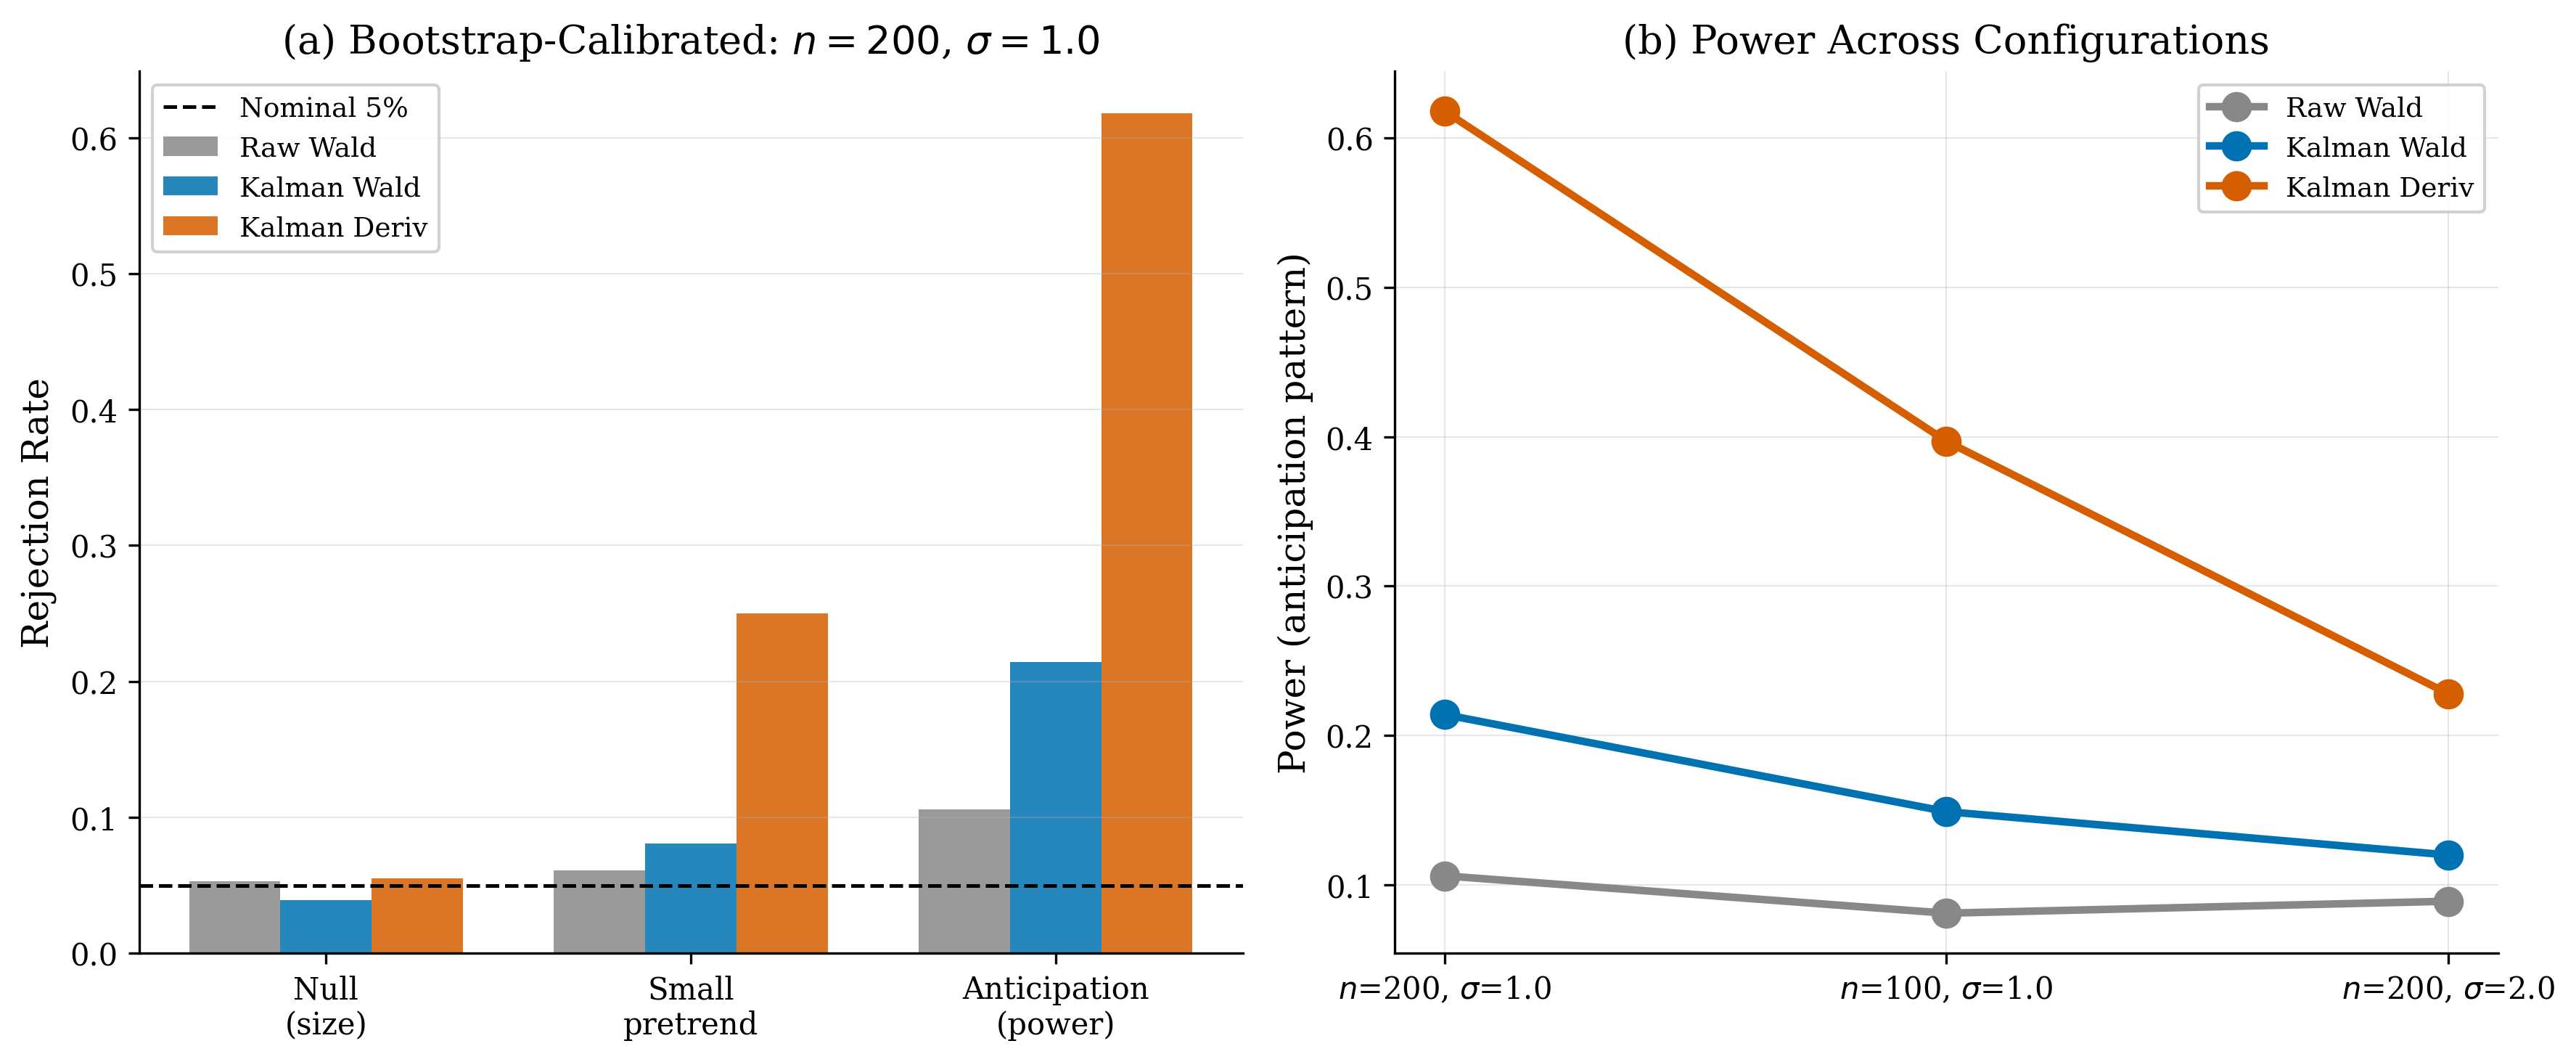
\includegraphics[width=\textwidth]{../figs/paper_fig3.png}
\caption{(a) Size and power at baseline. (b) Power against anticipation across configurations. The Kalman-based tests achieve modest but consistent power improvements while maintaining correct size.}
\label{fig:sizepower}
\end{figure}


\subsection{Sensitivity to Process Noise $\mathbf{Q}$}\label{sec:sensitivity}

\begin{table}[H]
\centering
\caption{Sensitivity to $\mathbf{Q}$ ($N = 200$, $\sigma = 1$, gradual pattern)}\label{tab:sensitivity}
\begin{tabular}{rr rr}
\toprule
$q_\ell$ & $q_s$ & Level MSE ($\times 10^3$) & Deriv MSE ($\times 10^3$) \\
\midrule
0.0005 & 0.0002 & 4.79 & 0.87 \\
0.0010 & 0.0005 & 4.62 & 0.83 \\
0.0020 & 0.0010 & 4.88 & 0.87 \\
0.0050 & 0.0020 & 5.60 & 0.96 \\
0.0100 & 0.0050 & 6.89 & 1.22 \\
0.0200 & 0.0100 & 8.54 & 1.50 \\
\bottomrule
\end{tabular}

\end{table}

Performance degrades gradually with misspecification of $\mathbf{Q}$ (Table~\ref{tab:sensitivity}, Figure~\ref{fig:sensitivity}). Even a 10$\times$ misspecification yields MSE well below raw estimates. We recommend $q_\ell \in [0.001, 0.005]$ and $q_s \in [0.0005, 0.002]$ as practical defaults.

\begin{figure}[H]
\centering
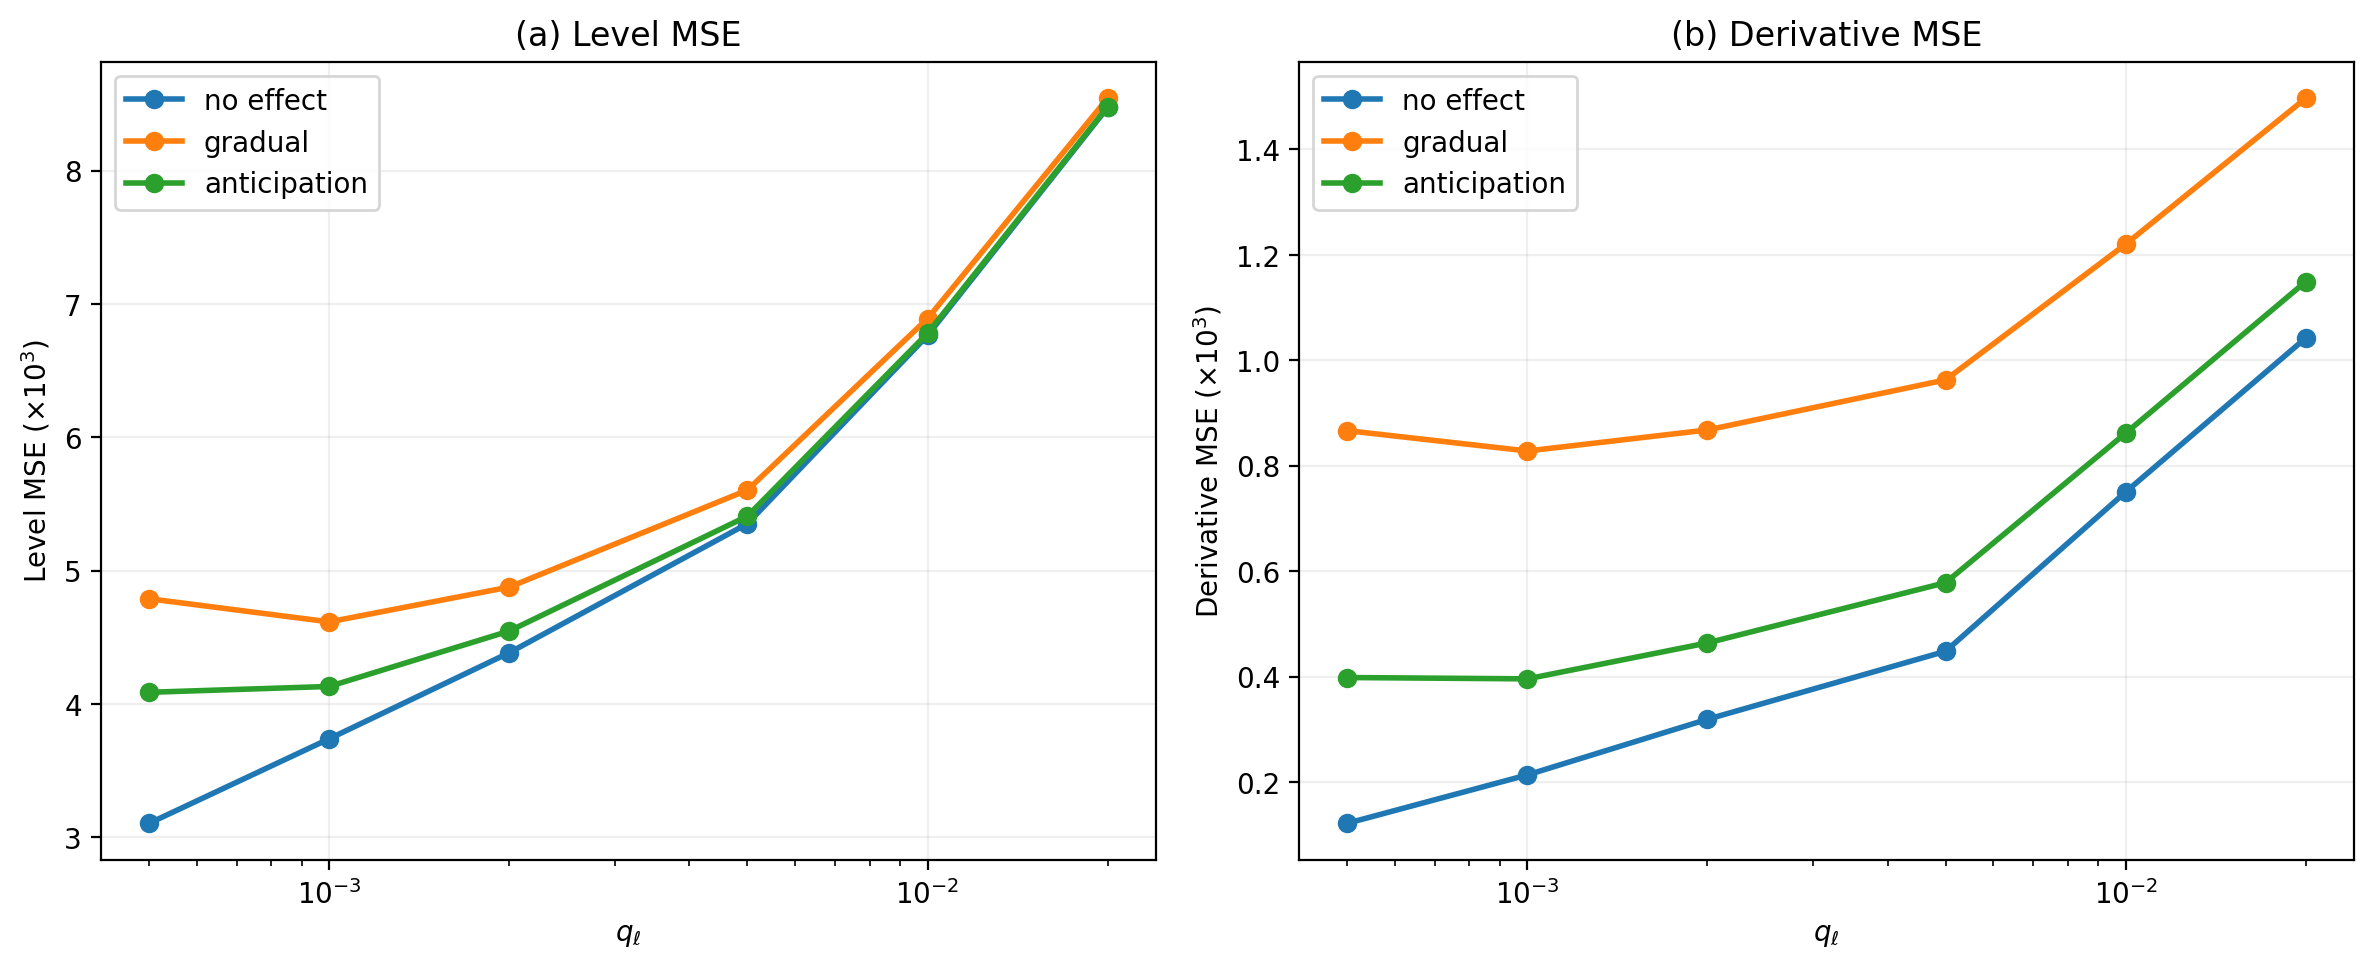
\includegraphics[width=\textwidth]{../figs/paper_fig4.png}
\caption{Level and derivative MSE as a function of $q_\ell$, for three treatment effect patterns.}
\label{fig:sensitivity}
\end{figure}

\subsection{Diagnostic Checks}\label{sec:diagnostics}

We recommend the following diagnostics before applying the Kalman smoother.

\paragraph{Independence.} Extract the variance-covariance matrix $\text{Var}(\hat{\boldsymbol\beta})$ from the TWFE regression. If $\max_{s \neq t}|\text{corr}(\hat{\beta}_s, \hat{\beta}_t)| > 0.1$, consider extending the observation model to use the full VCV rather than assuming diagonal noise.

\paragraph{Normality.} Q-Q plot the standardized residuals $\hat{\beta}_t / \hat{\sigma}_t$. With $\geq 30$ clusters, normality is typically satisfied by the CLT.

\paragraph{Smoothness.} Plot the standardized innovations $e_t = (\hat{\beta}_t - \mathbf{H} \hat{\mathbf{x}}_{t|t-1}) / \sqrt{S_t}$ from the Kalman filter forward pass. Under correct specification, these should be approximately i.i.d.\ $N(0,1)$. Positive autocorrelation in $e_t$ suggests $\mathbf{Q}$ is too small (undersmoothing); negative autocorrelation suggests $\mathbf{Q}$ is too large.

\paragraph{$\mathbf{Q}$ selection via marginal likelihood.} The marginal log-likelihood
\begin{equation}
\log L(\mathbf{Q}) = -\frac{1}{2} \sum_{t=1}^T \left( \log S_t + e_t^2 / S_t \right)
\end{equation}
can be maximized over $\mathbf{Q}$ to select the process noise automatically, eliminating the tuning parameter. This is the approach taken in state-space model estimation \citep{durbin2012time}.


\section{Discussion and Limitations}\label{sec:limitations}

\paragraph{When the approach works best.} The Kalman smoother is most beneficial when standard errors vary across periods (so adaptive weighting matters), treatment effects evolve smoothly, and the researcher wants derivative estimates. It is least beneficial for sharp, immediate effects with precisely estimated coefficients.

\paragraph{The smoothness prior and sharp effects.} For the immediate pattern, the smoother still reduces level MSE by 70\%, but attenuates the jump and propagates some post-treatment signal backward. The bootstrap calibration accounts for this and maintains correct size.

\paragraph{Independence across periods.} Assumption~\ref{a:normal} requires independence of $\hat{\beta}_t$ across $t$. Extensions incorporating correlated observation noise are straightforward but require estimating the autocorrelation.

\paragraph{Why not empirical Bayes?} EB shrinks toward zero. This is optimal under no effect but harmful under treatment: it pulls the trajectory toward the wrong target. The Kalman smoother shrinks toward a smooth trajectory---a more appropriate prior when treatment effects are nonzero but evolving.

\paragraph{Why not parametric trends?} A linear trend model works when the pre-trend is linear, but fails catastrophically otherwise (MSE 4$\times$ worse than raw for the gradual pattern). The Kalman smoother's nonparametric flexibility avoids this risk.

\paragraph{Pre-testing concerns.} \citet{roth2022pretest} shows that conditioning on passing a pre-test distorts inference. Our test detects slightly more violations, though the power gains are modest. However, violations that survive our test are precisely those the smoother has shrunk the most, raising questions about the interaction between power gains and conditioning bias that warrant further investigation.

\paragraph{Comparison with \citet{rambachan2023more}.} Our approach and Rambachan--Roth address different aspects of the parallel trends problem. They provide sensitivity analysis for bounded violations; we provide better estimates of the treatment effect trajectory. The Kalman-smoothed estimates could serve as inputs to their framework, potentially yielding tighter bounds.

\paragraph{Choice of $\mathbf{Q}$.} This is a tuning parameter analogous to bandwidth in nonparametric regression. Marginal likelihood maximization, cross-validation, or calibration to the observed $\hat{\beta}_t$ variability are all viable selection methods.

\section{Conclusion}

Event study coefficient sequences are noisy observations of a smooth latent process with known, heteroskedastic measurement error. The Kalman smoother is the optimal linear estimator for this setting, and substantially outperforms competitive baselines---including James--Stein shrinkage, empirical Bayes, and Savitzky--Golay---for both level and derivative estimation. The MSE gains are particularly large for derivative estimation (98\% reduction), enabling researchers to visualize and interpret treatment effect dynamics with much greater precision. For parallel trends testing, the Kalman-based tests achieve correct size via parametric bootstrap and modest power improvements over the standard Wald test. The primary contribution is thus in \emph{estimation}---recovering smooth trajectories and their derivatives from noisy event study coefficients---rather than dramatic power gains for hypothesis testing.

\bibliographystyle{apalike}
\bibliography{references}

\end{document}
